\documentclass[11pt,letterpaper]{article}

% ============================================================================
% PACKAGES
% ============================================================================
\usepackage[utf8]{inputenc}
\usepackage[T1]{fontenc}
\usepackage{helvet}
\renewcommand{\familydefault}{\sfdefault}
\usepackage[margin=0.85in, headheight=28pt]{geometry}
\usepackage{graphicx}
\usepackage{xcolor}
\usepackage{tikz}
\usepackage{tcolorbox}
\usepackage{booktabs}
\usepackage{enumitem}
\usepackage{hyperref}
\usepackage{fancyhdr}
\usepackage{titlesec}
\usepackage{multicol}
\usepackage{listings}
\usepackage{upquote}
\usepackage{amsmath,amssymb}
\usepackage{pgfplots}
\usepackage{array}
\usepackage{longtable}

% Ragged-right paragraph columns to prevent word spacing issues
\newcolumntype{L}[1]{>{\raggedright\arraybackslash}p{#1}}

% Increase vertical spacing between table rows for readability
\renewcommand{\arraystretch}{1.4}

\usepackage{colortbl}
\usepackage{pifont}
\usepackage{setspace}
\usepackage{parskip}
\usepackage{caption}

\pgfplotsset{compat=1.18}
\usetikzlibrary{shapes.geometric, arrows.meta, positioning, calc, decorations.pathreplacing, backgrounds, fit, shadows.blur, matrix, patterns, fadings, shadings}

% ============================================================================
% COLOR DEFINITIONS - Modern AWS/Cloud Palette
% ============================================================================
\definecolor{awsdark}{HTML}{161E2D}         % Deep navy
\definecolor{awsblue}{HTML}{232F3E}         % AWS dark blue
\definecolor{awsorange}{HTML}{FF9900}       % AWS signature orange
\definecolor{awslightorange}{HTML}{FFAC33}  % Lighter orange
\definecolor{cloudblue}{HTML}{4A90D9}       % Sky blue
\definecolor{cloudlight}{HTML}{E8F4FD}      % Light cloud
\definecolor{successgreen}{HTML}{2ECC71}    % Success green
\definecolor{warningamber}{HTML}{F39C12}    % Warning amber
\definecolor{dangerred}{HTML}{E74C3C}       % Danger red
\definecolor{infoteal}{HTML}{17A2B8}        % Info teal
\definecolor{coolgray}{HTML}{6C757D}        % Cool gray
\definecolor{lightgray}{HTML}{F8F9FA}       % Light background
\definecolor{codebg}{HTML}{F7F7F7}          % Light code background
\definecolor{codetext}{HTML}{333333}        % Dark code text
\definecolor{codekeyword}{HTML}{0000FF}     % Blue keywords
\definecolor{codestring}{HTML}{008000}      % Green strings
\definecolor{codecomment}{HTML}{808080}     % Gray comments
\definecolor{codenumber}{HTML}{098658}      % Teal numbers
\definecolor{codeborder}{HTML}{E0E0E0}      % Border color

% ============================================================================
% HYPERREF SETUP
% ============================================================================
\hypersetup{
  colorlinks=true,
  linkcolor=cloudblue,
  urlcolor=awsorange,
  pdftitle={AgentCore Memory Integration Guide (Rust + ChromaDB)},
  pdfauthor={AI Agent Team}
}

% ============================================================================
% SPACING AND TYPOGRAPHY
% ============================================================================
\setstretch{1.15}
\setlength{\parskip}{0.5em}
\setlist{nosep, leftmargin=1.5em, itemsep=0.3em}

% ============================================================================
% PAGE STYLE
% ============================================================================
\pagestyle{fancy}
\fancyhf{}
\fancyhead[L]{%
  \begin{tikzpicture}[baseline=-0.5ex]
    \fill[awsorange] (0,0) circle (0.15);
    \fill[awsorange!70] (0.35,0) circle (0.1);
    \fill[awsorange!40] (0.6,0) circle (0.06);
  \end{tikzpicture}
  \hspace{0.3em}\textcolor{awsblue}{\textsf{\textbf{AgentCore Memory}}}%
}
\fancyhead[R]{\textcolor{coolgray}{\textsf{\thepage}}}
\fancyfoot[C]{\textcolor{coolgray}{\small\textsf{AgentCore Memory Integration Guide (Rust + ChromaDB)}}}
\renewcommand{\headrulewidth}{0pt}
\renewcommand{\footrulewidth}{0pt}

% Add subtle top border
\fancyheadoffset{0pt}
\setlength{\headheight}{32pt}

% ============================================================================
% SECTION FORMATTING - Modern Style
% ============================================================================
\titleformat{\section}
  {\normalfont\LARGE\bfseries\color{awsblue}}
  {\colorbox{awsorange}{\textcolor{white}{\thesection}}}{0.8em}{}
\titleformat{\subsection}
  {\normalfont\Large\bfseries\color{awsblue!80}}
  {\thesubsection}{0.6em}{}
\titleformat{\subsubsection}
  {\normalfont\large\color{coolgray}\bfseries}
  {\thesubsubsection}{0.5em}{}

\titlespacing*{\section}{0pt}{3ex plus 1ex minus .2ex}{2ex plus .2ex}
\titlespacing*{\subsection}{0pt}{2.5ex plus 1ex minus .2ex}{1.5ex plus .2ex}

% ============================================================================
% TOC STYLING
% ============================================================================
\setcounter{tocdepth}{2}

% ============================================================================
% TCOLORBOX ENVIRONMENTS - Modern Redesign
% ============================================================================
\tcbuselibrary{skins,breakable,hooks}

% Key Concept Box - Gradient left border
\newtcolorbox{keybox}[1][Key Concept]{
  enhanced,
  breakable,
  colback=cloudlight,
  colframe=cloudblue,
  colbacktitle=cloudblue,
  coltitle=white,
  fonttitle=\bfseries\sffamily,
  title={\faLightbulb\hspace{0.5em}#1},
  boxrule=0pt,
  leftrule=4pt,
  arc=0pt,
  outer arc=0pt,
  left=12pt, right=12pt, top=8pt, bottom=8pt,
  shadow={2pt}{-2pt}{0pt}{black!20}
}

% Warning Box - Bold left accent
\newtcolorbox{warnbox}[1][Warning]{
  enhanced,
  breakable,
  colback=dangerred!5,
  colframe=dangerred,
  colbacktitle=dangerred,
  coltitle=white,
  fonttitle=\bfseries\sffamily,
  title={\faExclamationTriangle\hspace{0.5em}#1},
  boxrule=0pt,
  leftrule=4pt,
  arc=0pt,
  outer arc=0pt,
  left=12pt, right=12pt, top=8pt, bottom=8pt,
  shadow={2pt}{-2pt}{0pt}{black!15}
}

% Success/Tip Box
\newtcolorbox{tipbox}[1][Pro Tip]{
  enhanced,
  breakable,
  colback=successgreen!8,
  colframe=successgreen,
  colbacktitle=successgreen,
  coltitle=white,
  fonttitle=\bfseries\sffamily,
  title={\faCheckCircle\hspace{0.5em}#1},
  boxrule=0pt,
  leftrule=4pt,
  arc=0pt,
  outer arc=0pt,
  left=12pt, right=12pt, top=8pt, bottom=8pt,
  shadow={2pt}{-2pt}{0pt}{black!15}
}

% AWS Service Box - Orange accent
\newtcolorbox{awsbox}[1][AWS Service]{
  enhanced,
  breakable,
  colback=awsorange!5,
  colframe=awsorange,
  colbacktitle=awsorange,
  coltitle=white,
  fonttitle=\bfseries\sffamily,
  title={\faAws\hspace{0.5em}#1},
  boxrule=0pt,
  leftrule=4pt,
  arc=0pt,
  outer arc=0pt,
  left=12pt, right=12pt, top=8pt, bottom=8pt,
  shadow={2pt}{-2pt}{0pt}{black!15}
}

% Info Box - Teal accent
\newtcolorbox{infobox}[1][Note]{
  enhanced,
  breakable,
  colback=infoteal!5,
  colframe=infoteal,
  colbacktitle=infoteal,
  coltitle=white,
  fonttitle=\bfseries\sffamily,
  title={\faInfoCircle\hspace{0.5em}#1},
  boxrule=0pt,
  leftrule=4pt,
  arc=0pt,
  outer arc=0pt,
  left=12pt, right=12pt, top=8pt, bottom=8pt,
  shadow={2pt}{-2pt}{0pt}{black!15}
}

% TL;DR Summary Box - Prominent
\newtcolorbox{tldrbox}{
  enhanced,
  breakable,
  colback=awsblue!3,
  colframe=awsblue,
  boxrule=1.5pt,
  arc=8pt,
  outer arc=8pt,
  left=15pt, right=15pt, top=12pt, bottom=12pt,
  fontupper=\small,
  before upper={\textcolor{awsorange}{\faRocket}\hspace{0.5em}\textbf{TL;DR}\hspace{0.8em}},
  shadow={3pt}{-3pt}{0pt}{black!20}
}

% ============================================================================
% CODE LISTING STYLE - Light Theme for Readability
% ============================================================================
\lstdefinelanguage{Rust}{
  morekeywords={async,await,fn,pub,struct,impl,enum,match,let,mut,self,Self,use,mod,crate,super,trait,where,for,in,if,else,return,true,false,Some,None,Ok,Err,Result,Option,Vec,String,HashMap,Arc,RwLock,Box,dyn},
  sensitive=true,
  morecomment=[l]{//},
  morecomment=[s]{/*}{*/},
  morestring=[b]",
}
\lstdefinestyle{moderncode}{
  language=Rust,
  basicstyle=\ttfamily\small\color{codetext},
  keywordstyle=\color{codekeyword}\bfseries,
  stringstyle=\color{codestring},
  commentstyle=\color{codecomment}\itshape,
  backgroundcolor=\color{codebg},
  frame=single,
  rulecolor=\color{codeborder},
  framesep=8pt,
  numbers=left,
  numberstyle=\tiny\color{coolgray},
  numbersep=12pt,
  breaklines=true,
  showstringspaces=false,
  tabsize=4,
  xleftmargin=25pt,
  framexleftmargin=20pt,
  aboveskip=1em,
  belowskip=1em,
  literate={`}{\`}1
}
\lstset{style=moderncode}

% Custom caption format for listings
\DeclareCaptionFormat{codecaption}{%
  \begin{tcolorbox}[
    enhanced,
    colback=awsblue!5,
    colframe=awsblue!50,
    boxrule=0.5pt,
    arc=4pt,
    left=8pt, right=8pt, top=4pt, bottom=4pt,
    before skip=0pt,
    after skip=0.5em
  ]
  \textcolor{awsblue}{\faFileCode}\hspace{0.5em}\small\sffamily #1#2#3
  \end{tcolorbox}
}
\captionsetup[lstlisting]{format=codecaption, labelfont={bf}, textfont={}, skip=0pt}

% ============================================================================
% ICON COMMANDS (pifont replacements for fontawesome5)
% ============================================================================
\newcommand{\faRobot}{\ding{70}}
\newcommand{\faCheck}{\ding{51}}
\newcommand{\faCheckCircle}{\ding{51}}
\newcommand{\faTimes}{\ding{55}}
\newcommand{\faTimesCircle}{\ding{55}}
\newcommand{\faExclamationTriangle}{\ding{74}}
\newcommand{\faExclamationCircle}{\ding{74}}
\newcommand{\faLightbulb}{\ding{72}}
\newcommand{\faInfoCircle}{\ding{73}}
\newcommand{\faRocket}{\ding{228}}
\newcommand{\faDatabase}{\ding{115}}
\newcommand{\faTachometerAlt}{\ding{99}}
\newcommand{\faAws}{\textbf{AWS}}
\newcommand{\faCloud}{\ding{110}}
\newcommand{\faBrain}{\ding{70}}
\newcommand{\faServer}{\ding{115}}
\newcommand{\faProjectDiagram}{\ding{118}}
\newcommand{\faLayerGroup}{\ding{115}}
\newcommand{\faCode}{\texttt{</>}}
\newcommand{\faCogs}{\ding{70}}
\newcommand{\faShieldAlt}{\ding{110}}
\newcommand{\faKey}{\ding{70}}
\newcommand{\faEye}{\ding{70}}
\newcommand{\faCloudUploadAlt}{\ding{110}}
\newcommand{\faChartLine}{\ding{70}}
\newcommand{\faDollarSign}{\$}
\newcommand{\faBook}{\ding{70}}
\newcommand{\faFileCode}{\ding{70}}
\newcommand{\faPython}{\ding{70}}
\newcommand{\faGithub}{\ding{70}}
\newcommand{\faListAlt}{\ding{70}}
\newcommand{\faClock}{\ding{70}}
\newcommand{\faSearch}{\ding{70}}
\newcommand{\faCog}{\ding{70}}
\newcommand{\faSquare}{\ding{111}}
\newcommand{\faCalculator}{\ding{70}}
\newcommand{\faBan}{\ding{55}}
\newcommand{\faFileAlt}{\ding{70}}
\newcommand{\faRandom}{\ding{70}}
\newcommand{\faEraser}{\ding{70}}
\newcommand{\faLock}{\ding{70}}
\newcommand{\faUserShield}{\ding{70}}
\newcommand{\faRust}{\ding{70}}
\newcommand{\faDocker}{\ding{70}}

% ============================================================================
% CUSTOM COMMANDS
% ============================================================================
\newcommand{\api}[1]{\texttt{\textcolor{cloudblue}{#1}}}
\newcommand{\code}[1]{\texttt{\small\colorbox{lightgray}{#1}}}
\newcommand{\ratelimit}{\textcolor{dangerred}{\faExclamationCircle\ 0.25 req/sec}}

% ============================================================================
% PART PAGE STYLING (uses explicit dimensions, not remember picture overlay)
% ============================================================================
\newcommand{\partpage}[4]{%
  \clearpage
  \thispagestyle{empty}
  \vspace*{-0.85in}
  \noindent\hspace*{-0.85in}\begin{tikzpicture}
    % Header background
    \shade[top color=awsdark, bottom color=awsblue]
      (0,0) rectangle (\paperwidth, -9cm);

    % Decorative circles
    \fill[awsorange, opacity=0.15] (12cm, -3cm) circle (4cm);
    \fill[awsorange, opacity=0.1] (14cm, -6cm) circle (2.5cm);
    \fill[cloudblue, opacity=0.1] (3cm, -5cm) circle (3cm);

    % Part number - large watermark
    \node[white, opacity=0.08, font=\fontsize{200}{200}\selectfont\bfseries]
      at (5cm, -5cm) {#1};

    % Part label
    \node[white, font=\large\sffamily] at (0.5\paperwidth, -2.5cm) {PART};

    % Part number (visible)
    \node[awsorange, font=\fontsize{72}{72}\selectfont\bfseries]
      at (0.5\paperwidth, -4.5cm) {#1};

    % Part title
    \node[white, font=\Huge\bfseries\sffamily] at (0.5\paperwidth, -7cm) {#2};

    % Decorative line
    \draw[awsorange, line width=2pt]
      (3cm, -8cm) -- (\paperwidth-3cm, -8cm);
  \end{tikzpicture}

  \vspace{0.8cm}

  % Overview content
  \begin{center}
  \begin{minipage}{0.88\textwidth}
    \begin{tcolorbox}[
      enhanced,
      colback=white,
      colframe=awsorange!50,
      boxrule=1pt,
      arc=6pt,
      left=15pt, right=15pt, top=12pt, bottom=12pt,
      shadow={2pt}{-2pt}{0pt}{black!15}
    ]
    \textcolor{awsblue}{\faListAlt\hspace{0.5em}\textbf{What's Covered}}
    \vspace{0.5em}

    #3
    \end{tcolorbox}

    \vspace{1em}

    % Icon row
    \begin{center}
    #4
    \end{center}
  \end{minipage}
  \end{center}
}

% ============================================================================
% DOCUMENT
% ============================================================================
\begin{document}

% ============================================================================
% TITLE PAGE - Full Page Design with remember picture
% ============================================================================
\begin{titlepage}

\begin{tikzpicture}[remember picture, overlay]
  % Left panel gradient (full height)
  \shade[left color=awsdark, right color=awsblue!90]
    (current page.north west) rectangle ([xshift=7cm]current page.south west);

  % Decorative circles on left panel
  \fill[awsorange, opacity=0.15] ([xshift=3.5cm, yshift=-4cm]current page.north west) circle (1.2cm);
  \fill[awsorange, opacity=0.10] ([xshift=3.5cm, yshift=-8cm]current page.north west) circle (0.9cm);
  \fill[cloudblue, opacity=0.12] ([xshift=3.5cm, yshift=-12cm]current page.north west) circle (1.1cm);
  \fill[awsorange, opacity=0.08] ([xshift=3.5cm, yshift=-16cm]current page.north west) circle (1.4cm);
  \fill[cloudblue, opacity=0.10] ([xshift=3.5cm, yshift=-20cm]current page.north west) circle (0.8cm);

  % Memory hub visualization centered at left panel
  \begin{scope}[shift={([xshift=3.5cm, yshift=-14cm]current page.north west)}]
    % Glow rings
    \fill[awsorange, opacity=0.08] (0,0) circle (2.8cm);
    \fill[awsorange, opacity=0.12] (0,0) circle (2.2cm);

    % Central hub
    \fill[awsorange] (0,0) circle (0.65cm);
    \node[white, font=\small\bfseries] at (0,0) {MEM};

    % Agent nodes around hub
    \foreach \angle/\label/\col in {60/C/cloudblue, 120/G/successgreen, 180/O/infoteal, 240/X/warningamber, 300/R/dangerred, 0/P/coolgray} {
      \draw[white, opacity=0.4, line width=1.5pt] (0,0) -- (\angle:1.6cm);
      \fill[\col] (\angle:2cm) circle (0.35cm);
      \node[white, font=\tiny\bfseries] at (\angle:2cm) {\label};
    }

    % Data particles
    \foreach \i in {1,...,12} {
      \fill[white, opacity=0.5] ({30*\i}:1cm) circle (0.05cm);
    }
  \end{scope}

  % ========== RIGHT SIDE CONTENT ==========

  % Platform Badge
  \node[fill=awsorange, rounded corners=3pt, inner sep=6pt]
    at ([xshift=11cm, yshift=-3cm]current page.north west)
    {\textcolor{white}{\small\bfseries\sffamily RUST + CHROMADB}};

  % Main Title
  \node[anchor=west] at ([xshift=8cm, yshift=-5.5cm]current page.north west) {
    {\fontsize{48}{54}\selectfont\bfseries\color{awsblue}AgentCore}
  };
  \node[anchor=west] at ([xshift=8cm, yshift=-7.5cm]current page.north west) {
    {\fontsize{38}{44}\selectfont\color{cloudblue}Memory}
  };
  \node[anchor=west] at ([xshift=8cm, yshift=-9cm]current page.north west) {
    {\Large\color{coolgray}\sffamily Integration Guide}
  };

  % Tagline
  \node[anchor=west] at ([xshift=8cm, yshift=-11cm]current page.north west) {
    {\large\color{awsblue}\sffamily Persistent Memory for AI Agent Ecosystems}
  };

  % Orange divider
  \draw[awsorange, line width=3pt]
    ([xshift=8cm, yshift=-12cm]current page.north west) --
    ([xshift=18cm, yshift=-12cm]current page.north west);

  % Description
  \node[anchor=north west, text width=10cm] at ([xshift=8cm, yshift=-13cm]current page.north west) {
    \color{coolgray}\normalsize
    Enable your AI agents to remember context across sessions, share knowledge,
    and leverage semantic search---all self-hosted with ChromaDB and a Rust MCP server.
  };

  % Feature highlights
  \node[fill=cloudblue!10, rounded corners=4pt, inner sep=8pt]
    at ([xshift=9.5cm, yshift=-16.5cm]current page.north west) {
    \textcolor{cloudblue}{\faBrain}\hspace{0.3em}\small\sffamily Short-Term Events
  };
  \node[fill=successgreen!10, rounded corners=4pt, inner sep=8pt]
    at ([xshift=13.5cm, yshift=-16.5cm]current page.north west) {
    \textcolor{successgreen}{\faDatabase}\hspace{0.3em}\small\sffamily Long-Term Facts
  };
  \node[fill=awsorange!10, rounded corners=4pt, inner sep=8pt]
    at ([xshift=17.5cm, yshift=-16.5cm]current page.north west) {
    \textcolor{awsorange}{\faSearch}\hspace{0.3em}\small\sffamily Semantic Search
  };

  % Rate limit indicators
  \node[fill=dangerred!10, rounded corners=3pt, inner sep=6pt]
    at ([xshift=10cm, yshift=-19cm]current page.north west) {
    \textcolor{dangerred}{\faTimes}\hspace{0.3em}\scriptsize\sffamily Rate Limited
  };
  \node[fill=successgreen!10, rounded corners=3pt, inner sep=6pt]
    at ([xshift=14cm, yshift=-19cm]current page.north west) {
    \textcolor{successgreen}{\faCheck}\hspace{0.3em}\scriptsize\sffamily No Limit
  };

  % Version info
  \node[coolgray, font=\sffamily] at ([xshift=13cm, yshift=-21cm]current page.north west) {
    Version 1.0 | December 4, 2025
  };
\end{tikzpicture}
\end{titlepage}

% ============================================================================
% EXECUTIVE SUMMARY
% ============================================================================
\newpage
\thispagestyle{empty}

\begin{center}
{\color{awsblue}\fontsize{28}{32}\selectfont\bfseries Executive Summary}
\end{center}

\vspace{1cm}

\begin{tldrbox}
AI agents are stateless. This integration adds persistent memory via a Rust MCP server backed by ChromaDB,
enabling cross-session context and shared knowledge across your entire agent ecosystem.
\end{tldrbox}

\vspace{1.5em}

% Enhanced Problem/Solution/Constraint cards with side icons
\begin{tikzpicture}
  \node[fill=dangerred!8, rounded corners=10pt, text width=0.88\textwidth, inner sep=15pt, anchor=north west,
        drop shadow={shadow xshift=2pt, shadow yshift=-2pt, opacity=0.15}] (prob) at (1.2,0) {
    \textcolor{dangerred}{\textbf{THE PROBLEM}}\\[0.5em]
    \color{awsblue}AI agents (Claude Code, Gemini, OpenCode, Crush, Codex) lose all context between sessions.
    Each conversation starts from scratch---no memory of codebase patterns, user preferences, or prior learnings.
  };
  % Side icon
  \node[fill=dangerred, circle, minimum size=1cm, inner sep=0pt] at (0.4, -0.7) {
    \textcolor{white}{\large\faBrain}
  };
\end{tikzpicture}

\vspace{0.8em}

\begin{tikzpicture}
  \node[fill=successgreen!8, rounded corners=10pt, text width=0.88\textwidth, inner sep=15pt, anchor=north west,
        drop shadow={shadow xshift=2pt, shadow yshift=-2pt, opacity=0.15}] at (1.2,0) {
    \textcolor{successgreen}{\textbf{THE SOLUTION}}\\[0.5em]
    \color{awsblue}A Rust MCP server with ChromaDB provides self-hosted short-term and long-term memory.
    All agents connect via the MCP protocol to a local persistent vector store.
  };
  % Side icon
  \node[fill=successgreen, circle, minimum size=1cm, inner sep=0pt] at (0.4, -0.7) {
    \textcolor{white}{\large\faCloud}
  };
\end{tikzpicture}

\vspace{0.8em}

\begin{tikzpicture}
  \node[fill=awsorange!8, rounded corners=10pt, text width=0.88\textwidth, inner sep=15pt, anchor=north west,
        drop shadow={shadow xshift=2pt, shadow yshift=-2pt, opacity=0.15}] at (1.2,0) {
    \textcolor{awsorange}{\textbf{KEY CONSTRAINT}}\\[0.5em]
    \color{awsblue}ChromaDB has \textbf{no rate limits}, but the MCP server is designed for sparse, high-value events.
    Store goals, decisions, and outcomes---not every conversation turn.
    Secret sanitization prevents accidental storage of API keys and tokens.
  };
  % Side icon
  \node[fill=awsorange, circle, minimum size=1cm, inner sep=0pt] at (0.4, -0.7) {
    \textcolor{white}{\large\faTachometerAlt}
  };
\end{tikzpicture}

\vspace{1.5em}

% API Overview Table
\begin{center}
\renewcommand{\arraystretch}{1.4}
\begin{tabular}{L{3.5cm} >{\centering\arraybackslash}p{5cm} L{5.5cm}}
\rowcolor{awsblue!10}
\textbf{\color{awsblue}Memory Type} & \textbf{\color{awsblue}API} & \textbf{\color{awsblue}Use Case} \\
\midrule
Short-term events & \api{CreateEvent} \textcolor{dangerred}{\tiny(0.25/s)} & Session goals, key decisions \\
Long-term facts & \api{BatchCreateMemoryRecords} & Patterns, preferences, learnings \\
Semantic search & \api{RetrieveMemoryRecords} & Context retrieval by meaning \\
\bottomrule
\end{tabular}
\end{center}

\vspace{2em}

% Architecture Preview
\begin{center}
\begin{tikzpicture}[
  layer/.style={rectangle, rounded corners=6pt, minimum height=1.2cm, font=\small\sffamily},
  arrow/.style={->, thick, >=stealth, awsblue!70}
]
  % Agents layer
  \node[layer, fill=cloudlight, draw=cloudblue, minimum width=12cm] (agents) at (0,2) {
    \faRobot\ \ Claude \quad\faRobot\ \ Gemini \quad\faRobot\ \ OpenCode \quad\faRobot\ \ Crush \quad\faRobot\ \ Codex
  };

  % MCP layer
  \node[layer, fill=awsblue!10, draw=awsblue, minimum width=12cm] (mcp) at (0,0) {
    \textbf{mcp-agentcore-memory} \textcolor{coolgray}{(Rust, ChromaDB)}
  };

  % Storage layer
  \node[layer, fill=awsorange!10, draw=awsorange, minimum width=12cm] (aws) at (0,-2) {
    \faDatabase\ \ ChromaDB (Vector Store)
  };

  \draw[arrow] (agents) -- (mcp);
  \draw[arrow, awsorange] (mcp) -- node[right, font=\tiny, color=coolgray] {HTTP} (aws);

  % Labels
  \node[coolgray, font=\tiny, anchor=east] at ([xshift=-0.5cm]agents.west) {Self-Hosted};
  \node[coolgray, font=\tiny, anchor=east] at ([xshift=-0.5cm]aws.west) {Self-Hosted};
\end{tikzpicture}
\end{center}

% ============================================================================
% TABLE OF CONTENTS
% ============================================================================
\newpage
\tableofcontents
\newpage

% ============================================================================
% CRITICAL CORRECTIONS FROM EXTERNAL REVIEWS
% ============================================================================
\section*{\faExclamationTriangle\ Critical Corrections from External Reviews}
\addcontentsline{toc}{section}{Critical Corrections}

\begin{warnbox}[This Section Documents Breaking Changes!]
Two external reviews identified critical issues that \textbf{fundamentally changed} the implementation approach. Review this section before implementing.
\end{warnbox}

\vspace{1em}

\subsection*{First Review: Hard Blockers}

\begin{center}
\renewcommand{\arraystretch}{1.5}
\begin{tabular}{L{3cm} L{4.5cm} L{6cm}}
\rowcolor{dangerred!15}
\textbf{\color{dangerred}Issue} & \textbf{\color{dangerred}Impact} & \textbf{\color{dangerred}Resolution} \\
\midrule
\rowcolor{lightgray}
Rate limits wrong & CreateEvent is 0.25 req/sec per actor+session (not 100 TPS). ``Store every turn'' will throttle immediately. & Store coarse-grained events only; use BatchCreateMemoryRecords for facts \\
Control vs Data plane & CreateMemory is control plane, events are data plane. PrivateLink doesn't cover control plane. & Use separate clients; accept control plane uses public endpoint \\
\rowcolor{lightgray}
API shapes wrong & Response paths, payload formats don't match actual AWS APIs & Rewrite client to match actual API docs \\
async + boto3 = blocking & boto3 is synchronous; will stall MCP server under load & Resolved: migrated to Rust async with ChromaDB backend \\
\bottomrule
\end{tabular}
\end{center}

\vspace{1.5em}

\subsection*{Second Review: Implementation Fixes}

\begin{center}
\renewcommand{\arraystretch}{1.5}
\begin{tabular}{L{3.5cm} L{4cm} L{6cm}}
\rowcolor{warningamber!15}
\textbf{\color{warningamber}Issue} & \textbf{\color{warningamber}Impact} & \textbf{\color{warningamber}Resolution} \\
\midrule
\rowcolor{lightgray}
CreateEvent payload shape & Code will 400---branchName (string) vs branch (struct) & Fixed: \code{branch=\{"name": ...\}}, payload as list of unions \\
RetrieveMemoryRecords query & API requires searchQuery; empty fails & Fixed: query parameter now required; added separate list method \\
\rowcolor{lightgray}
Rate limiter not keyed & Global limiter doesn't match per-session limit & Fixed: \code{PerSessionRateLimiter} keyed by (actor\_id, session\_id) \\
Restore uses CreateEvent & Would take forever at 0.25/s & Fixed: Use BatchCreateMemoryRecords for restore \\
\rowcolor{lightgray}
Tests mock boto3 & Implementation uses aiobotocore; tests give false confidence & Resolved: Rust unit tests with direct assertions (no mocking needed) \\
Sanitize patterns incomplete & Missing AWS keys, GitHub tokens & Fixed: Added AKIA pattern, gh[pousr]\_ pattern, entropy detection \\
\bottomrule
\end{tabular}
\end{center}

\vspace{1.5em}

\subsection*{Third Review: Real AWS Integration Testing (2025-12)}

\begin{center}
\renewcommand{\arraystretch}{1.5}
\begin{tabular}{L{3.8cm} L{4cm} L{5.7cm}}
\rowcolor{successgreen!15}
\textbf{\color{successgreen}Issue} & \textbf{\color{successgreen}Impact} & \textbf{\color{successgreen}Resolution} \\
\midrule
\rowcolor{lightgray}
BatchCreate param name & API expects \code{records}, not \code{memoryRecords} & Fixed: Changed parameter name \\
BatchCreate record structure & Requires \code{requestIdentifier}, \code{namespaces} (list), \code{timestamp} & Fixed: Added all required fields \\
\rowcolor{lightgray}
BatchCreate response shape & Returns \code{successfulRecords}/\code{failedRecords}, not \code{memoryRecords}/\code{errors} & Fixed: Updated response parsing \\
RetrieveRecords searchCriteria & Uses \code{searchQuery} (string), not \code{semanticQuery} (struct) & Fixed: Changed to simple string \\
\rowcolor{lightgray}
eventExpiryDuration units & Value is in DAYS (max 365), not ISO 8601 duration & Fixed: Changed to integer days \\
Memory name constraints & Must match \code{[a-zA-Z][a-zA-Z0-9\_]\{0,47\}} (no dashes!) & Fixed in setup script \\
\bottomrule
\end{tabular}
\end{center}

\vspace{1.5em}

\subsection*{Design Philosophy Changes}

\begin{center}
\begin{tikzpicture}[
  box/.style={rectangle, rounded corners=8pt, minimum width=6.5cm, minimum height=2.5cm,
    font=\small\sffamily, align=left, text width=6cm, inner sep=10pt}
]
  % Original design (crossed out)
  \node[box, fill=dangerred!10, draw=dangerred] (orig) at (-4, 0) {
    \textbf{\color{dangerred}\faTimes\ Original (Wrong)}\\[0.5em]
    \textcolor{coolgray}{\textbullet\ \code{store\_event} for every turn}\\
    \textcolor{coolgray}{\textbullet\ 100 TPS assumption}\\
    \textcolor{coolgray}{\textbullet\ ``100 MB = \$0.50'' pricing}\\
    \textcolor{coolgray}{\textbullet\ PrivateLink everywhere}
  };

  % Final design (ChromaDB)
  \node[box, fill=successgreen!10, draw=successgreen] (corr) at (4, 0) {
    \textbf{\color{successgreen}\faCheck\ Final (ChromaDB)}\\[0.5em]
    \textcolor{awsblue}{\textbullet\ Sparse events: goals, decisions, outcomes}\\
    \textcolor{awsblue}{\textbullet\ No rate limits (self-hosted)}\\
    \textcolor{awsblue}{\textbullet\ Zero cloud cost}\\
    \textcolor{awsblue}{\textbullet\ Local Docker volume persistence}
  };

  % Arrow
  \draw[->, very thick, awsorange, >=stealth] (orig) -- (corr);
\end{tikzpicture}
\end{center}

\newpage

% ============================================================================
% PART I: ARCHITECTURE
% ============================================================================
\partpage{I}{Architecture}{%
\begin{itemize}[leftmargin=1.5em]
  \item \textbf{Section 1:} Current state analysis---why agents forget everything
  \item \textbf{Section 2:} Proposed architecture with Rust MCP server and ChromaDB
  \item \textbf{Section 3:} Multi-provider abstraction for flexibility
\end{itemize}
}{%
\textcolor{cloudblue}{\faCode}\quad
\textcolor{awsorange}{\faCogs}\quad
\textcolor{successgreen}{\faTachometerAlt}
}

\section{Current State Analysis}

\begin{tldrbox}
All agents are stateless. No memory persists. Agents can't share knowledge. This limits effectiveness on long-running projects.
\end{tldrbox}

\subsection{The Stateless Agent Problem}

\begin{keybox}[Core Problem]
Current AI agents operate in \textbf{isolated sessions}:
\begin{itemize}
  \item Each session starts with zero context about the codebase
  \item Learnings from PR reviews vanish after the review ends
  \item User preferences must be re-established every time
  \item Agents cannot benefit from each other's discoveries
\end{itemize}
\end{keybox}

\vspace{1em}

% Visual diagram of the problem
\begin{center}
\begin{tikzpicture}[
  agent/.style={rectangle, rounded corners=8pt, fill=cloudlight, draw=cloudblue,
    minimum width=2.8cm, minimum height=1.2cm, font=\small\bfseries\sffamily},
  mcp/.style={rectangle, rounded corners=6pt, fill=awsblue!8, draw=awsblue!50,
    minimum width=10cm, minimum height=1cm, font=\small\sffamily},
  problem/.style={rectangle, rounded corners=8pt, fill=dangerred!10, draw=dangerred,
    text width=8cm, align=center, inner sep=10pt, font=\small},
  arrow/.style={->, thick, cloudblue!70, >=stealth}
]
  % Agents
  \node[agent] (claude) at (0, 2.5) {\faRobot\ Claude};
  \node[agent] (gemini) at (4, 2.5) {\faRobot\ Gemini};
  \node[agent] (opencode) at (8, 2.5) {\faRobot\ OpenCode};

  % MCP layer
  \node[mcp] (mcp) at (4, 0.5) {MCP Servers (code-quality, github-board, ...)};

  % Arrows
  \draw[arrow] (claude) -- (mcp);
  \draw[arrow] (gemini) -- (mcp);
  \draw[arrow] (opencode) -- (mcp);

  % Problem callout
  \node[problem] at (4, -1.8) {
    \textcolor{dangerred}{\faTimesCircle}\quad\textbf{No persistent memory layer!}\\[0.3em]
    Agents forget everything between sessions.
  };

  % Dashed line showing gap
  \draw[dashed, dangerred, thick] (0, -0.5) -- (8, -0.5);
\end{tikzpicture}
\end{center}

\subsection{Goals and Non-Goals}

\begin{multicols}{2}
\begin{tipbox}[Goals]
\begin{itemize}
  \item Cross-session memory for all agents
  \item Shared knowledge base
  \item Semantic search for retrieval
  \item Self-hosted ChromaDB backend
\end{itemize}
\end{tipbox}

\columnbreak

\begin{warnbox}[Non-Goals]
\begin{itemize}
  \item Replace GitHub Board for coordination
  \item Depend on cloud services
  \item Auto-inject context (explicit only)
  \item \textcolor{dangerred}{Log every conversation turn!}
\end{itemize}
\end{warnbox}
\end{multicols}

\section{Proposed Architecture}

\begin{tldrbox}
Rust MCP server using ChromaDB for vector storage and semantic search. SHA-256 namespace hashing for collection names. LRU cache with TTL for query performance.
\end{tldrbox}

\subsection{System Overview}

\begin{center}
\begin{tikzpicture}[
  infra/.style={rectangle, rounded corners=8pt, draw=awsblue, fill=awsblue!3,
    minimum width=13cm, minimum height=5cm},
  aws/.style={rectangle, rounded corners=8pt, draw=awsorange, fill=awsorange!3,
    minimum width=13cm, minimum height=3.5cm},
  agent/.style={rectangle, rounded corners=6pt, fill=cloudlight, draw=cloudblue,
    minimum width=2.2cm, minimum height=1cm, font=\scriptsize\bfseries\sffamily},
  mcpbox/.style={rectangle, rounded corners=6pt, fill=awsblue!15, draw=awsblue,
    minimum width=11cm, minimum height=1.3cm, font=\small\sffamily},
  membox/.style={rectangle, rounded corners=6pt, minimum width=4.5cm, minimum height=1.8cm, font=\scriptsize\sffamily, align=center},
  arrow/.style={->, thick, >=stealth}
]
  % Infrastructure box
  \node[infra] (infra) at (0, 2.5) {};
  \node[awsblue, font=\small\bfseries, anchor=north west] at ([xshift=0.5cm, yshift=-0.3cm]infra.north west) {
    \faServer\ Self-Hosted Infrastructure
  };

  % Agents
  \node[agent] (c) at (-4.5, 3.5) {\faRobot\ Claude};
  \node[agent] (g) at (-1.5, 3.5) {\faRobot\ Gemini};
  \node[agent] (o) at (1.5, 3.5) {\faRobot\ OpenCode};
  \node[agent] (x) at (4.5, 3.5) {\faRobot\ Codex};

  % MCP Server
  \node[mcpbox] (mcp) at (0, 1.5) {\textbf{mcp-agentcore-memory} \textcolor{coolgray}{(Rust async, ChromaDB)}};

  % Arrows to MCP
  \foreach \n in {c,g,o,x} {
    \draw[arrow, cloudblue!70] (\n) -- (mcp);
  }

  % AWS box
  \node[aws] (awsbox) at (0, -2) {};
  \node[awsorange, font=\small\bfseries, anchor=north west] at ([xshift=0.5cm, yshift=-0.3cm]awsbox.north west) {
    \faDatabase\ ChromaDB Vector Store
  };

  % Memory types
  \node[membox, fill=infoteal!10, draw=infoteal] (short) at (-3, -2.3) {
    \textbf{Short-Term Memory}\\[0.2em]
    \api{store\_event}\\[0.2em]
    \textcolor{successgreen}{\tiny\faCheckCircle\ No rate limit}
  };

  \node[membox, fill=successgreen!10, draw=successgreen] (long) at (3, -2.3) {
    \textbf{Long-Term Memory}\\[0.2em]
    \api{store\_facts}\\[0.2em]
    \textcolor{successgreen}{\tiny\faCheckCircle\ No rate limit}
  };

  % Arrow from MCP to ChromaDB
  \draw[arrow, awsorange, line width=2pt] (mcp) -- node[right, font=\scriptsize, color=coolgray] {HTTP} (awsbox.north);
\end{tikzpicture}
\end{center}

\subsection{ChromaDB Client Architecture}

\begin{infobox}[Single Client Design]
The Rust MCP server uses a single \code{ChromaDBClient} that communicates with ChromaDB over HTTP. Unlike the original AWS design (which required separate control/data plane clients), ChromaDB provides a unified REST API for all operations---collections, documents, and queries.
\end{infobox}

\subsection{Memory Lifecycle Flow}

\begin{center}
\begin{tikzpicture}[
  stage/.style={rectangle, rounded corners=10pt, minimum width=2.8cm, minimum height=1.8cm,
    font=\small\sffamily, align=center, drop shadow={shadow xshift=2pt, shadow yshift=-2pt, opacity=0.2}},
  arrow/.style={->, thick, >=stealth, line width=1.5pt},
  label/.style={font=\tiny\sffamily, color=coolgray}
]
  % Stage 1: Agent Input
  \node[stage, fill=cloudlight, draw=cloudblue] (input) at (0,0) {
    \faRobot\\[2pt]\textbf{Agent}\\[-2pt]\textbf{Input}
  };

  % Stage 2: Sanitization
  \node[stage, fill=dangerred!10, draw=dangerred] (sanitize) at (3.5,0) {
    \faShieldAlt\\[2pt]\textbf{Sanitize}\\[-2pt]\textbf{Secrets}
  };

  % Stage 3: Rate Limiter
  \node[stage, fill=warningamber!15, draw=warningamber] (ratelimit) at (7,0) {
    \faTachometerAlt\\[2pt]\textbf{Rate}\\[-2pt]\textbf{Limiter}
  };

  % Stage 4: Short-term
  \node[stage, fill=infoteal!15, draw=infoteal] (shortterm) at (10.5,0) {
    \faClock\\[2pt]\textbf{Short-Term}\\[-2pt]\textbf{Events}
  };

  % Stage 5: Long-term (below)
  \node[stage, fill=successgreen!15, draw=successgreen] (longterm) at (10.5,-3) {
    \faDatabase\\[2pt]\textbf{Long-Term}\\[-2pt]\textbf{Facts}
  };

  % Arrows
  \draw[arrow, cloudblue] (input) -- (sanitize);
  \draw[arrow, dangerred] (sanitize) -- node[above, label] {clean} (ratelimit);
  \draw[arrow, warningamber] (ratelimit) -- node[above, label] {0.25/s} (shortterm);
  \draw[arrow, successgreen, dashed] (shortterm) -- node[right, label, text width=1.5cm, align=center] {extraction\\consolidation} (longterm);

  % Retrieval arrow back
  \draw[arrow, cloudblue!60, dashed] (longterm.west) -- ++(-7,0) |- node[near start, below, label] {semantic search} (input.south);

  % Rate limit indicator
  \node[fill=dangerred!80, text=white, font=\tiny\bfseries, rounded corners=3pt, inner sep=3pt]
    at ([yshift=-0.5cm]ratelimit.south) {THROTTLED};
  \node[fill=successgreen!80, text=white, font=\tiny\bfseries, rounded corners=3pt, inner sep=3pt]
    at ([yshift=-0.5cm]longterm.south) {NO LIMIT};
\end{tikzpicture}
\end{center}

\section{Provider Abstraction}

\begin{tldrbox}
The original design included an abstract \code{MemoryProvider} interface for multi-backend support. The current implementation uses ChromaDB exclusively, which provides zero-cost self-hosted operation.
\end{tldrbox}

\subsection{Provider Comparison}

\begin{center}
\renewcommand{\arraystretch}{1.6}
\begin{tabular}{L{3.5cm} c c}
\rowcolor{awsblue}
\textbf{\color{white}Feature} & \textbf{\color{white}AWS AgentCore} & \textbf{\color{white}ChromaDB} \\
\rowcolor{lightgray}
Managed service & \textcolor{successgreen}{\faCheckCircle} & \textcolor{coolgray}{\faTimesCircle} \\
Self-hosted option & \textcolor{coolgray}{\faTimesCircle} & \textcolor{successgreen}{\faCheckCircle} \\
\rowcolor{lightgray}
Rate limits & \textcolor{dangerred}{0.25/s} & \textcolor{successgreen}{None} \\
Cost & Per-record & Free \\
\rowcolor{lightgray}
Enterprise ready & \textcolor{successgreen}{\faCheckCircle} & \textcolor{warningamber}{\faExclamationCircle} \\
\bottomrule
\end{tabular}
\end{center}

\subsection{Provider Interface}

All providers implement a common interface for seamless switching:

\begin{lstlisting}[caption={Memory provider architecture (Rust)}]
/// The current implementation uses ChromaDB directly.
/// A trait-based provider abstraction can be added when
/// multiple backends are needed.
pub struct ChromaDBClient {
    http_client: reqwest::Client,
    config: ChromaDBConfig,
    collections: RwLock<HashMap<String, String>>,
}

impl ChromaDBClient {
    /// Store a short-term event.
    pub async fn store_event(
        &self, actor_id: &str, session_id: &str, content: &str,
    ) -> Result<String, String> { /* ... */ }

    /// Semantic search across memories.
    pub async fn search(
        &self, query: &str, namespace: &str, top_k: u32,
    ) -> Result<Vec<MemoryRecord>, String> { /* ... */ }

    /// Batch store long-term facts.
    pub async fn store_facts(
        &self, facts: &[String], namespace: &str,
    ) -> Result<Vec<String>, String> { /* ... */ }

    /// Check provider connectivity.
    pub async fn health_check(&self) -> Result<bool, String> { /* ... */ }
}
\end{lstlisting}

\subsection{ChromaDB Provider (Zero-Cost Development)}

ChromaDB provides a self-hosted vector database perfect for development and testing:

\begin{lstlisting}[caption={ChromaDB client implementation (Rust)}]
pub struct ChromaDBConfig {
    pub host: String,     // default: "localhost"
    pub port: u16,        // default: 8000
    pub collection: String, // default: "agent_memory"
}

impl ChromaDBClient {
    pub fn new(config: ChromaDBConfig) -> Self {
        Self {
            http_client: reqwest::Client::builder()
                .timeout(Duration::from_secs(30))
                .build().unwrap(),
            config,
            collections: RwLock::new(HashMap::new()),
        }
    }

    /// Collection names use SHA-256 hashing for stable,
    /// collision-free mapping from namespace to ChromaDB name.
    fn collection_name(&self, namespace: &str) -> String {
        let hash = sha256(namespace);
        format!("{}_rec_{:x}", self.config.collection, &hash[..8])
    }

    pub async fn search(
        &self, query: &str, namespace: &str, top_k: u32,
    ) -> Result<Vec<MemoryRecord>, String> {
        let collection_id = self.get_or_create_collection(namespace).await?;
        let body = json!({
            "query_texts": [query],
            "n_results": top_k,
        });
        let resp = self.http_client
            .post(format!("{}/api/v1/collections/{}/query",
                self.base_url(), collection_id))
            .json(&body)
            .send().await?;
        // Parse and return results...
    }
}
\end{lstlisting}

\begin{tipbox}[ChromaDB Benefits]
\begin{itemize}
  \item \textbf{Zero cost}: No cloud fees, runs locally
  \item \textbf{No rate limits}: Store as frequently as needed
  \item \textbf{Fast iteration}: Perfect for development/testing
  \item \textbf{Easy migration}: Export to production later
\end{itemize}
\end{tipbox}

\begin{keybox}[Provider Selection Guide]
\begin{itemize}
  \item \textbf{Development/Self-hosted}: ChromaDB (zero cost, no rate limits, full control)
  \item \textbf{Enterprise/managed}: AWS AgentCore (fully managed, IAM, compliance)
\end{itemize}
Toggle via \code{MEMORY\_PROVIDER} environment variable.
\end{keybox}

\section{Integration Points}

\begin{tldrbox}
Memory integrates with Claude Code via MCP, GitHub Agents via direct client calls, and Gemini via pre-search context injection. Each agent uses the shared memory for cross-session learning.
\end{tldrbox}

\subsection{Claude Code Configuration}

Add the memory server to \code{.mcp.json}:

\begin{lstlisting}[caption={MCP configuration for Claude Code}, language={}]
{
  "mcpServers": {
    "agentcore-memory": {
      "command": "docker compose",
      "args": [
        "-f", "./docker-compose.yml",
        "run", "--rm", "-T", "mcp-agentcore-memory"
      ],
      "env": {
        "CHROMADB_HOST": "${CHROMADB_HOST:-localhost}",
        "CHROMADB_PORT": "${CHROMADB_PORT:-8000}"
      }
    }
  }
}
\end{lstlisting}

\begin{tipbox}[Usage Patterns for Claude Code]
\begin{itemize}
  \item \textbf{Session start}: ``Search memories for patterns related to authentication''
  \item \textbf{After learning}: ``Store this fact: The API uses JWT with 15-min expiry''
  \item \textbf{During PR work}: ``Store event: PR \#47 changes OAuth2 flow''
  \item \textbf{Cross-session}: ``What did I learn about testing patterns?''
\end{itemize}
\end{tipbox}

\subsection{GitHub Agents Integration}

Issue Monitor and PR Monitor agents use memory for context-aware processing:

\begin{center}
\begin{tikzpicture}[
  agent/.style={rectangle, rounded corners=6pt, fill=cloudlight, draw=cloudblue,
    minimum width=3.2cm, minimum height=1.2cm, font=\small\sffamily},
  stepbox/.style={rectangle, rounded corners=4pt, fill=awsorange!10, draw=awsorange,
    minimum width=2.5cm, minimum height=0.8cm, font=\scriptsize\sffamily},
  arrow/.style={->, thick, >=stealth, awsblue}
]
  % Issue Monitor flow
  \node[agent] (issue) at (0, 0) {Issue Monitor};
  \node[stepbox] (recall) at (4.5, 0.5) {Recall similar issues};
  \node[stepbox] (process) at (4.5, -0.5) {Process with context};
  \node[stepbox] (store) at (9, 0) {Store learnings};

  \draw[arrow] (issue) -- (recall);
  \draw[arrow] (issue) -- (process);
  \draw[arrow] (recall) -- (store);
  \draw[arrow] (process) -- (store);

  \node[coolgray, font=\tiny] at (4.5, -1.3) {\code{search\_memories(query=issue.title)}};
  \node[coolgray, font=\tiny] at (9, -0.7) {\code{store\_facts([summary])}};
\end{tikzpicture}
\end{center}

\subsection{Gemini Review Integration}

Gemini uses memory to recall codebase conventions before generating reviews:

\begin{lstlisting}[caption={Pre-populating review context from memory}, language={}]
// search_memories MCP tool call
{
  "query": "coding conventions and style guidelines",
  "namespace": "codebase/conventions",
  "top_k": 10
}

// Agent uses returned memories in its review prompt:
// "Review this PR considering these established conventions:
//  <memories>
//  Diff: <pr_diff>"
\end{lstlisting}

\section{Memory Strategies}

\begin{tldrbox}
AgentCore supports automatic extraction from short-term events and manual storage for explicit facts. Use automatic for sessions, manual for high-confidence learnings.
\end{tldrbox}

\subsection{Automatic Extraction}

Short-term events are processed by configurable extraction strategies:

\begin{center}
\renewcommand{\arraystretch}{1.5}
\begin{tabular}{L{3cm} L{5cm} L{5cm}}
\rowcolor{infoteal!15}
\textbf{\color{infoteal}Strategy} & \textbf{\color{infoteal}What It Extracts} & \textbf{\color{infoteal}Use Case} \\
\midrule
\rowcolor{lightgray}
Semantic & Facts, entities, relationships & Codebase knowledge, patterns \\
Summarization & Conversation summaries & Session context, decisions \\
\rowcolor{lightgray}
User Preference & Expressed preferences & Coding style, tool choices \\
\bottomrule
\end{tabular}
\end{center}

\subsection{Manual Extraction}

For high-confidence learnings, use \code{store\_facts} directly:

\begin{lstlisting}[caption={Explicit fact storage after successful work}, language={}]
// store_facts MCP tool call
{
  "facts": ["The data layer uses Repository pattern with async SQLAlchemy"],
  "namespace": "codebase/architecture",
  "source": "PR #42 - Data layer refactoring"
}
\end{lstlisting}

% ============================================================================
% PART II: IMPLEMENTATION
% ============================================================================
\newpage
\partpage{II}{Implementation}{%
\begin{itemize}[leftmargin=1.5em]
  \item \textbf{Section 4:} Rust MCP server design (ChromaDB backend)
  \item \textbf{Section 5:} API payload shapes and collection naming
  \item \textbf{Section 6:} Caching and sanitization strategy
\end{itemize}
}{%
\textcolor{cloudblue}{\faCode}\quad
\textcolor{awsorange}{\faCogs}\quad
\textcolor{successgreen}{\faTachometerAlt}
}

\section{MCP Server Design}

\begin{tldrbox}
The \code{mcp-agentcore-memory} server exposes 6 tools for memory operations. It uses ChromaDB as the vector database backend with an LRU cache, content sanitization, and namespace-aware collection management.
\end{tldrbox}

\subsection{MCP Tools Specification}

\begin{center}
\renewcommand{\arraystretch}{1.5}
\begin{tabular}{L{3.5cm} L{4.5cm} L{5.5cm}}
\rowcolor{cloudblue!15}
\textbf{\color{cloudblue}Tool Name} & \textbf{\color{cloudblue}Description} & \textbf{\color{cloudblue}Key Parameters} \\
\midrule
\rowcolor{lightgray}
\code{store\_event} & Store short-term event & \code{content}, \code{actor\_id}, \code{session\_id} \\
\code{store\_facts} & Batch store long-term facts & \code{facts[]}, \code{namespace}, \code{source} \\
\rowcolor{lightgray}
\code{search\_memories} & Semantic search across memories & \code{query}, \code{namespace}, \code{top\_k} \\
\code{list\_session\_events} & List events from a session & \code{actor\_id}, \code{session\_id}, \code{limit} \\
\rowcolor{lightgray}
\code{list\_namespaces} & List all 23 predefined namespaces & --- \\
\code{memory\_status} & Service status and cache stats & --- \\
\bottomrule
\end{tabular}
\end{center}

\begin{tipbox}[Use \code{store\_facts} for Long-Term Knowledge]
The \code{store\_facts} tool uses \api{BatchCreateMemoryRecords} internally, which has \textbf{no rate limit}. This is the preferred method for storing codebase patterns, architecture decisions, and learned preferences.
\end{tipbox}

\subsection{Namespace Design}

Namespaces organize memories by domain. Use consistent namespaces across agents for shared knowledge:

\begin{center}
\begin{tikzpicture}[
  ns/.style={rectangle, rounded corners=4pt, fill=#1!15, draw=#1,
    minimum height=0.8cm, font=\small\ttfamily, inner sep=6pt},
  cat/.style={font=\small\bfseries\sffamily, color=#1}
]
  % Codebase
  \node[cat=cloudblue] at (-5, 2) {Codebase};
  \node[ns=cloudblue] at (-5, 1.2) {codebase/architecture};
  \node[ns=cloudblue] at (-5, 0.3) {codebase/patterns};
  \node[ns=cloudblue] at (-5, -0.6) {codebase/conventions};

  % Preferences
  \node[cat=successgreen] at (0, 2) {Preferences};
  \node[ns=successgreen] at (0, 1.2) {preferences/user};
  \node[ns=successgreen] at (0, 0.3) {preferences/project};

  % Reviews
  \node[cat=awsorange] at (5, 2) {Reviews};
  \node[ns=awsorange] at (5, 1.2) {reviews/pr};
  \node[ns=awsorange] at (5, 0.3) {reviews/issues};

  % Agents
  \node[cat=infoteal] at (0, -1.5) {Agent-Specific};
  \node[ns=infoteal] at (-2, -2.3) {agents/claude};
  \node[ns=infoteal] at (2, -2.3) {agents/gemini};
\end{tikzpicture}
\end{center}

\subsection{Directory Structure}

\begin{lstlisting}[caption={MCP Server package layout (Rust)}, language={}]
tools/mcp/mcp_agentcore_memory/
+-- Cargo.toml                  # mcp-agentcore-memory crate
+-- src/
|   +-- main.rs                 # Entry point, CLI args, server init
|   +-- server.rs               # MCP tool implementations (6 tools)
|   +-- client.rs               # ChromaDB HTTP client abstraction
|   +-- types.rs                # Data structures, predefined namespaces
|   +-- cache.rs                # LRU memory cache with TTL
|   +-- sanitize.rs             # Secret detection and sanitization
\end{lstlisting}

\section{Memory Client Implementation}

\begin{keybox}[Rust + ChromaDB Architecture]
The Rust implementation communicates with ChromaDB via its REST API using \code{reqwest}. All I/O is async with Tokio. Collections are managed via SHA-256 namespace hashing for stable, collision-free names.
\end{keybox}

\subsection{Store Event Implementation}

\begin{lstlisting}[caption={Store event with sanitization (Rust)}]
pub async fn store_event(
    &self,
    actor_id: &str,
    session_id: &str,
    content: &str,
) -> Result<String, String> {
    // Sanitize content before storage
    let sanitized = sanitize_content(content);

    let collection_id = self
        .get_or_create_collection("events").await?;

    let doc_id = Uuid::new_v4().to_string();
    let metadata = json!({
        "actor_id": actor_id,
        "session_id": session_id,
        "timestamp": Utc::now().to_rfc3339(),
    });

    self.http_client.post(format!(
        "{}/api/v1/collections/{}/add",
        self.base_url(), collection_id
    ))
    .json(&json!({
        "ids": [doc_id],
        "documents": [sanitized],
        "metadatas": [metadata],
    }))
    .send().await
    .map_err(|e| e.to_string())?;

    Ok(doc_id)
}
\end{lstlisting}

\subsection{RetrieveMemoryRecords}

\begin{warnbox}[searchQuery is REQUIRED]
The \api{searchQuery} parameter is \textbf{mandatory}---you cannot list all records without a query. Use \api{list\_memory\_records()} for enumeration instead.
\end{warnbox}

\section{Rate Limiting Strategy}

\begin{keybox}[Per-Session Rate Limiting]
The 0.25 req/sec limit is per \code{(actor\_id, session\_id)} pair, NOT global! Your rate limiter must be keyed by session:
\end{keybox}

% Visual rate limit explanation
\begin{center}
\begin{tikzpicture}[
  session/.style={rectangle, rounded corners=6pt, fill=cloudlight, draw=cloudblue,
    minimum width=3cm, minimum height=1.5cm, font=\small\sffamily},
  bucket/.style={rectangle, rounded corners=4pt, fill=awsorange!20, draw=awsorange,
    minimum width=1.5cm, minimum height=0.8cm, font=\tiny}
]
  \node[session, align=center] (s1) at (0, 0) {Session A\\[0.1em]\tiny actor: claude};
  \node[session, align=center] (s2) at (4.5, 0) {Session B\\[0.1em]\tiny actor: claude};
  \node[session, align=center] (s3) at (9, 0) {Session C\\[0.1em]\tiny actor: gemini};

  \node[bucket] at ([yshift=-1.5cm]s1.south) {0.25/s};
  \node[bucket] at ([yshift=-1.5cm]s2.south) {0.25/s};
  \node[bucket] at ([yshift=-1.5cm]s3.south) {0.25/s};

  \node[coolgray, font=\scriptsize] at (4.5, -2.5) {Each session has its own independent rate limit bucket};
\end{tikzpicture}
\end{center}

\begin{infobox}[No Rate Limiting Required]
Unlike AWS AgentCore (0.25 req/sec per actor+session), ChromaDB has \textbf{no rate limits}. The Rust implementation uses a conservative fetch buffer instead:
\end{infobox}

\begin{lstlisting}[caption={Fetch buffer for list operations (Rust)}]
const MAX_FETCH_LIMIT: u32 = 50_000;

pub async fn list_events(
    &self,
    actor_id: &str,
    session_id: &str,
    limit: u32,
) -> Result<Vec<MemoryEvent>, String> {
    // Clamp to prevent memory exhaustion
    let fetch_limit = limit.clamp(10_000, MAX_FETCH_LIMIT);
    // Query ChromaDB with actor/session filter...
}
\end{lstlisting}

\begin{tipbox}[ChromaDB Operational Notes]
\begin{itemize}
  \item No rate limits---store as frequently as needed
  \item 30-second HTTP timeout on all requests
  \item Cache invalidation is namespace-aware (invalidating a parent clears children)
  \item Large sessions ($>$50k events) may need pagination
\end{itemize}
\end{tipbox}

% ============================================================================
% PART III: SECURITY
% ============================================================================
\newpage
\partpage{III}{Security}{%
\begin{itemize}[leftmargin=1.5em]
  \item \textbf{Section 7:} Content sanitization and secret detection
  \item \textbf{Section 8:} IAM policies with least privilege
  \item \textbf{Section 9:} Monitoring and audit trails
\end{itemize}
}{%
\textcolor{cloudblue}{\faCode}\quad
\textcolor{awsorange}{\faCogs}\quad
\textcolor{successgreen}{\faTachometerAlt}
}

\section{Content Sanitization}

\begin{warnbox}[Never Store Secrets!]
AI agents regularly see API keys, tokens, and credentials in code. These must be \textbf{detected and redacted} before any memory storage operation.
\end{warnbox}

\vspace{0.5em}

% Security Layers Visual
\begin{center}
\begin{tikzpicture}[
  layer/.style={rectangle, rounded corners=6pt, minimum width=11cm, minimum height=1.4cm,
    font=\small\sffamily, align=center},
  arrow/.style={->, thick, >=stealth, coolgray}
]
  % Input
  \node[layer, fill=cloudlight, draw=cloudblue] (input) at (0, 4) {
    \faFileAlt\ \textbf{Raw Agent Content} \textcolor{coolgray}{\small (may contain secrets)}
  };

  % Layer 1: Regex
  \node[layer, fill=dangerred!8, draw=dangerred] (regex) at (0, 2.3) {
    \faCode\ \textbf{Layer 1: Regex Patterns} --- AWS keys, GitHub PATs, OpenAI keys, Private keys
  };

  % Layer 2: Entropy
  \node[layer, fill=warningamber!10, draw=warningamber] (entropy) at (0, 0.6) {
    \faRandom\ \textbf{Layer 2: Entropy Analysis} --- Detect unknown high-entropy strings ($H > 4.5$)
  };

  % Layer 3: Redaction
  \node[layer, fill=successgreen!10, draw=successgreen] (redact) at (0, -1.1) {
    \faEraser\ \textbf{Layer 3: Redaction Markers} --- \code{[REDACTED]} or \code{[HIGH\_ENTROPY\_REDACTED]}
  };

  % Output
  \node[layer, fill=successgreen!20, draw=successgreen, line width=1.5pt] (output) at (0, -2.8) {
    \faShieldAlt\ \textbf{Sanitized Content} \textcolor{successgreen}{\small (safe for storage)}
  };

  % Arrows
  \draw[arrow] (input) -- (regex);
  \draw[arrow] (regex) -- (entropy);
  \draw[arrow] (entropy) -- (redact);
  \draw[arrow, successgreen, line width=1.5pt] (redact) -- (output);

  % Side indicators
  \node[dangerred, font=\tiny, rotate=90] at (-6, 2.3) {DETECT};
  \node[warningamber, font=\tiny, rotate=90] at (-6, 0.6) {ANALYZE};
  \node[successgreen, font=\tiny, rotate=90] at (-6, -1.1) {REPLACE};
\end{tikzpicture}
\end{center}

\subsection{Detection Patterns}

\begin{center}
\renewcommand{\arraystretch}{1.5}
\begin{tabular}{L{3cm} >{\ttfamily\small\raggedright\arraybackslash}p{8cm}}
\rowcolor{dangerred}
\textbf{\color{white}Secret Type} & \textbf{\color{white}\textrm{Detection Pattern}} \\
\rowcolor{dangerred!5}
\faAws\ AWS Access Key & AKIA[0-9A-Z]\{16\} \\
\faGithub\ GitHub PAT & gh[pousr]\_[A-Za-z0-9\_]\{36,\} \\
\rowcolor{dangerred!5}
\faKey\ OpenAI Key & sk-[a-zA-Z0-9]\{20,\} \\
\faLock\ Private Keys & -----BEGIN.*PRIVATE KEY----- \\
\rowcolor{dangerred!5}
\faRandom\ High Entropy & \textrm{Shannon entropy $H > 4.5$} \\
\bottomrule
\end{tabular}
\end{center}

\begin{tipbox}[Defense in Depth]
The sanitization pipeline uses multiple layers:
\begin{enumerate}
  \item \textbf{Regex patterns} for known secret formats
  \item \textbf{Entropy analysis} for unknown high-entropy blobs
  \item \textbf{Explicit markers}: \code{[REDACTED]} or \code{[HIGH\_ENTROPY\_REDACTED]}
\end{enumerate}
\end{tipbox}

\subsection{Data Classification}

Not all data should be stored in memory. Follow this classification:

\begin{center}
\renewcommand{\arraystretch}{1.5}
\begin{tabular}{L{3.5cm} >{\centering\arraybackslash}p{2.5cm} L{6.5cm}}
\rowcolor{awsblue!15}
\textbf{\color{awsblue}Data Type} & \textbf{\color{awsblue}Sensitivity} & \textbf{\color{awsblue}Storage Policy} \\
\midrule
\rowcolor{lightgray}
Code patterns & Low & Long-term OK---store in \code{codebase/patterns} \\
Architecture decisions & Low & Long-term OK---valuable for consistency \\
\rowcolor{lightgray}
PR discussions & Low-Medium & Short-term only; summarize to facts \\
User preferences & Low & Long-term OK in \code{preferences/user} \\
\rowcolor{lightgray}
Issue context & Low-Medium & Extract key learnings; discard details \\
\rowcolor{dangerred!10}
Secrets/credentials & \textcolor{dangerred}{\textbf{NEVER}} & Block at client level---sanitize before storage \\
\rowcolor{dangerred!10}
API keys/tokens & \textcolor{dangerred}{\textbf{NEVER}} & Auto-redacted by sanitization pipeline \\
\rowcolor{dangerred!10}
PII/user data & \textcolor{dangerred}{\textbf{NEVER}} & Do not store personal information \\
\bottomrule
\end{tabular}
\end{center}

\begin{warnbox}[Storage Audit]
Periodically audit stored memories for accidentally-stored secrets:
\begin{enumerate}
  \item Export memories using backup script
  \item Scan exports with secret detection tools (trufflehog, git-secrets)
  \item Delete any records containing sensitive data
\end{enumerate}
\end{warnbox}

\section{Infrastructure Setup}

\subsection{Prerequisites}

\begin{keybox}[Before You Begin]
\begin{itemize}
  \item Docker and Docker Compose installed
  \item Rust toolchain (for building from source) or pre-built binary
  \item Available port 8000 for ChromaDB
\end{itemize}
\end{keybox}

\subsection{ChromaDB Setup}

ChromaDB is set up automatically via Docker Compose. Collections are created on first use---no manual provisioning needed:

\begin{lstlisting}[caption={ChromaDB setup via Docker Compose}, language={}]
# docker-compose.yml (ChromaDB service)
services:
  chromadb:
    image: chromadb/chroma:latest
    ports:
      - "8000:8000"
    volumes:
      - chromadb_data:/chroma/chroma
    environment:
      - IS_PERSISTENT=TRUE

  mcp-agentcore-memory:
    build: ./tools/mcp/mcp_agentcore_memory
    environment:
      - CHROMADB_HOST=chromadb
      - CHROMADB_PORT=8000
    depends_on:
      - chromadb
\end{lstlisting}

\begin{infobox}[No Cloud Dependencies]
ChromaDB runs locally as a Docker container---no AWS account, IAM roles, or API keys needed. All data stays on your self-hosted infrastructure, aligning with the project's container-first philosophy.
\end{infobox}

\section{Data Persistence}

ChromaDB stores data in a Docker volume (\code{chromadb\_data}). Collections are created automatically when the MCP server stores its first event for a namespace. Collection names are derived from SHA-256 hashes of the namespace string for safe cross-platform storage.

% ============================================================================
% PART IV: OPERATIONS
% ============================================================================
\newpage
\partpage{IV}{Operations}{%
\begin{itemize}[leftmargin=1.5em]
  \item \textbf{Section 10:} Backup and recovery strategies
  \item \textbf{Section 11:} Monitoring and alerting
  \item \textbf{Section 12:} Cost estimation and optimization
\end{itemize}
}{%
\textcolor{cloudblue}{\faCode}\quad
\textcolor{awsorange}{\faCogs}\quad
\textcolor{successgreen}{\faTachometerAlt}
}

\section{Backup and Recovery}

\begin{infobox}[ChromaDB Backup is Volume-Based]
Since ChromaDB stores all data in a Docker volume, backup and restore use standard Docker volume operations---no custom scripts needed.
\end{infobox}

\subsection{Volume Backup}

\begin{lstlisting}[caption={Backup ChromaDB Docker volume}, language={}]
# Stop the server to ensure consistency
docker compose stop chromadb

# Create a compressed backup of the volume
docker run --rm \
    -v chromadb_data:/data \
    -v $(pwd)/backups:/backup \
    alpine tar czf /backup/chromadb-$(date +%Y%m%d).tar.gz -C /data .

# Restart
docker compose up -d chromadb
\end{lstlisting}

\subsection{Volume Restore}

\begin{lstlisting}[caption={Restore ChromaDB from backup}, language={}]
# Stop all services using ChromaDB
docker compose stop chromadb mcp-agentcore-memory

# Restore volume from backup
docker run --rm \
    -v chromadb_data:/data \
    -v $(pwd)/backups:/backup \
    alpine sh -c "rm -rf /data/* && tar xzf /backup/chromadb-20260101.tar.gz -C /data"

# Restart services
docker compose up -d chromadb mcp-agentcore-memory
\end{lstlisting}

\begin{infobox}[Backup Schedule]
\begin{itemize}
  \item \textbf{Weekly full backup}: \code{0 0 * * 0 ./scripts/backup-chromadb.sh}
  \item \textbf{Store locally}: Keep backups on a separate drive or NAS
  \item \textbf{Test restores}: Quarterly restore to test environment
  \item \textbf{Retention}: Keep 4 weekly backups, 3 monthly backups
\end{itemize}
\end{infobox}

\section{Cost Estimation}

\begin{infobox}[Self-Hosted Pricing: Zero Cloud Cost]
ChromaDB is open-source and runs locally. The only costs are:
\begin{itemize}
  \item \textbf{Disk storage}: ChromaDB data volume (typically $<$1 GB for agent memory)
  \item \textbf{Compute}: Docker container overhead (minimal---ChromaDB is lightweight)
  \item \textbf{No API fees}: All operations are local, no per-request charges
\end{itemize}
\end{infobox}

\vspace{1em}

\begin{center}
\renewcommand{\arraystretch}{1.6}
\begin{tabular}{L{4cm} c r}
\rowcolor{awsorange}
\textbf{\color{white}Component} & \textbf{\color{white}Est. Volume} & \textbf{\color{white}Monthly Cost} \\
\rowcolor{lightgray}
\faDocker\ ChromaDB container & Persistent & \$0.00 \\
\faDatabase\ Storage volume & $<$1 GB & \$0.00 \\
\rowcolor{lightgray}
\faSearch\ Semantic searches & Unlimited & \$0.00 \\
\midrule
\rowcolor{successgreen!15}
\textbf{\faCalculator\ Total} & & \textbf{\textcolor{successgreen}{\$0.00}} \\
\bottomrule
\end{tabular}
\end{center}

\begin{tipbox}[Storage Optimization Tips]
\begin{itemize}
  \item Use \api{store\_facts} to consolidate short-term events into long-term knowledge
  \item The built-in LRU cache (1000 entries, 300s TTL) reduces redundant queries
  \item Namespace-aware invalidation keeps cache consistent with writes
\end{itemize}
\end{tipbox}

\section{Monitoring}

\begin{keybox}[Key Metrics to Track]
\begin{itemize}
  \item \textbf{Latency}: \code{store\_event\_latency}, \code{search\_memories\_latency}
  \item \textbf{Error rates}: Success/failure counts by operation type
  \item \textbf{ChromaDB health}: Monitor heartbeat endpoint and collection count
  \item \textbf{Cache effectiveness}: Local cache hit rate percentage
\end{itemize}
\end{keybox}

\subsection{Logging}

Use \code{RUST\_LOG} environment variable to control log verbosity. The MCP server logs all operations with timestamps:

\begin{lstlisting}[caption={Enable debug logging for troubleshooting}, language={}]
# In docker-compose.yml or environment
RUST_LOG=mcp_agentcore_memory=debug

# View logs
docker compose logs -f mcp-agentcore-memory
\end{lstlisting}

\subsection{Monitoring}

Use the \code{memory\_status} MCP tool to check server health, or query ChromaDB directly via its HTTP API:

\begin{lstlisting}[caption={Health check via ChromaDB API}, language={}]
# Check ChromaDB is responding
curl http://localhost:8000/api/v1/heartbeat

# List collections (one per namespace hash)
curl http://localhost:8000/api/v1/collections
\end{lstlisting}

\section{Latency and Caching}

Since ChromaDB runs locally alongside the MCP server, latency is minimal:

\begin{center}
\renewcommand{\arraystretch}{1.5}
\begin{tabular}{L{3.5cm} c L{6cm}}
\rowcolor{cloudblue!15}
\textbf{\color{cloudblue}Operation} & \textbf{\color{cloudblue}Expected Latency} & \textbf{\color{cloudblue}Mitigation} \\
\midrule
\rowcolor{lightgray}
\code{store\_event} & 5--20ms & Local ChromaDB write \\
\code{search\_memories} & 10--50ms & LRU cache with 5-min TTL \\
\rowcolor{lightgray}
\code{list\_session\_events} & 5--30ms & Session-scoped query \\
\bottomrule
\end{tabular}
\end{center}

\subsection{Local Cache Strategy}

\begin{lstlisting}[caption={LRU cache with TTL (Rust)}]
pub struct MemoryCache {
    entries: HashMap<String, CacheEntry>,
    max_size: usize,          // default: 1000
    ttl: Duration,            // default: 300s
}

impl MemoryCache {
    pub fn get(&mut self, query: &str, namespace: &str) -> Option<&Vec<MemoryRecord>> {
        let key = Self::make_key(query, namespace); // MD5 hash
        if let Some(entry) = self.entries.get_mut(&key) {
            if entry.timestamp.elapsed() < self.ttl {
                entry.timestamp = Instant::now(); // LRU update
                return Some(&entry.results);
            }
        }
        None
    }

    /// Namespace-aware invalidation
    pub fn invalidate(&mut self, namespace: Option<&str>) {
        match namespace {
            Some(ns) => self.entries.retain(|_, e| !e.namespace.starts_with(ns)),
            None => self.entries.clear(),
        }
    }
}
\end{lstlisting}

\subsection{Async Write Queue}

For resilient fire-and-forget writes, use an async queue with retry logic:

\begin{lstlisting}[caption={Cache flow in search\_memories (Rust)}]
impl MemoryServer {
    async fn handle_search(
        &self, query: &str, namespace: &str, top_k: u32,
    ) -> Result<Vec<MemoryRecord>, String> {
        // Fast path: check cache with read lock
        {
            let cache = self.cache.read().await;
            if let Some(results) = cache.get(query, namespace) {
                return Ok(results.clone());
            }
        }

        // Cache miss: query ChromaDB
        let results = self.client.search(query, namespace, top_k).await?;

        // Write results to cache
        {
            let mut cache = self.cache.write().await;
            cache.put(query, namespace, results.clone());
        }

        Ok(results)
    }
}
\end{lstlisting}

\begin{tipbox}[Queue Usage Pattern]
\begin{itemize}
  \item Use \code{enqueue()} for non-critical writes (session events)
  \item Call \code{flush()} before shutdown to ensure delivery
  \item Monitor \code{pending\_count()} for queue health
\end{itemize}
\end{tipbox}

\section{Testing Strategy}

\begin{keybox}[Rust Unit Tests]
The Rust implementation includes unit tests for sanitization, server creation, and tool registration. Integration tests require a running ChromaDB instance.
\end{keybox}

\subsection{Unit Test Pattern}

\begin{lstlisting}[caption={Rust unit tests for sanitization and server}]
#[cfg(test)]
mod tests {
    use super::*;

    #[test]
    fn test_sanitize_api_key() {
        let input = "Use key sk-abc123xyz for auth";
        let result = sanitize_content(input);
        assert!(result.contains("[REDACTED]"));
        assert!(!result.contains("sk-abc123xyz"));
    }

    #[test]
    fn test_high_entropy_detection() {
        let input = "token: aB3kL9mN2pQ5rS8tU1vW4xY7zA0bC6d";
        let (has_secrets, patterns) = contains_secrets(input);
        assert!(has_secrets);
        assert!(patterns.contains(&"high_entropy"));
    }

    #[tokio::test]
    async fn test_server_creation() {
        let server = MemoryServer::new(ChromaDBConfig::default());
        // Verify all 6 tools are registered
        assert_eq!(server.tools().len(), 6);
    }

    // Integration tests require: CHROMADB_HOST=localhost
    // docker compose up chromadb
    // cargo test -- --ignored
        "event": {"eventId": "evt-123"}
    }

    client = AgentCoreMemoryClient(config)
    with patch.object(client, "_get_data_plane_client", mock_context):
        result = await client.create_event(...)

    # Verify API shape
    call_kwargs = mock_client.create_event.call_args.kwargs
    assert "branch" in call_kwargs
    assert isinstance(call_kwargs["payload"], list)
\end{lstlisting}

\section{Rollout Plan}

\begin{center}
\begin{tikzpicture}[
  phase/.style={rectangle, rounded corners=8pt, minimum width=3.5cm, minimum height=2.5cm,
    font=\small\sffamily, align=center, text width=3.2cm},
  arrow/.style={->, very thick, >=stealth, awsorange}
]
  \node[phase, fill=cloudblue!15, draw=cloudblue] (p1) at (0, 0) {
    \textbf{Phase 1}\\[0.3em]
    Foundation\\[0.3em]
    {\tiny MCP server, client, tests}
  };
  \node[phase, fill=successgreen!15, draw=successgreen] (p2) at (4.5, 0) {
    \textbf{Phase 2}\\[0.3em]
    Claude Integration\\[0.3em]
    {\tiny MCP config, patterns}
  };
  \node[phase, fill=awsorange!15, draw=awsorange] (p3) at (9, 0) {
    \textbf{Phase 3}\\[0.3em]
    GitHub Agents\\[0.3em]
    {\tiny Issue/PR monitors}
  };
  \node[phase, fill=infoteal!15, draw=infoteal] (p4) at (13.5, 0) {
    \textbf{Phase 4}\\[0.3em]
    Hardening\\[0.3em]
    {\tiny Monitoring, docs}
  };

  \draw[arrow] (p1) -- (p2);
  \draw[arrow] (p2) -- (p3);
  \draw[arrow] (p3) -- (p4);
\end{tikzpicture}
\end{center}

\begin{keybox}[Phase 1 Checklist]
\begin{itemize}
  \item[\faSquare] Create \code{mcp\_agentcore\_memory} Rust crate structure
  \item[\faSquare] Implement \code{ChromaDBClient} with reqwest HTTP client
  \item[\faSquare] Implement MCP server with 6 core tools
  \item[\faSquare] Write unit tests (sanitization, cache, server creation)
  \item[\faSquare] Set up ChromaDB Docker service
\end{itemize}
\end{keybox}

\section{Infrastructure as Code}

\begin{tldrbox}
Docker Compose manages the entire stack. ChromaDB runs as a local container with persistent volumes---no cloud infrastructure required.
\end{tldrbox}

\subsection{Docker Compose Configuration}

\begin{lstlisting}[caption={Full Docker Compose for memory stack}, language={}]
# docker-compose.yml
services:
  chromadb:
    image: chromadb/chroma:latest
    ports:
      - "8000:8000"
    volumes:
      - chromadb_data:/chroma/chroma
    environment:
      - IS_PERSISTENT=TRUE
    healthcheck:
      test: ["CMD", "curl", "-f", "http://localhost:8000/api/v1/heartbeat"]
      interval: 30s
      timeout: 10s
      retries: 3

  mcp-agentcore-memory:
    build: ./tools/mcp/mcp_agentcore_memory
    environment:
      - CHROMADB_HOST=chromadb
      - CHROMADB_PORT=8000
      - RUST_LOG=info
    depends_on:
      chromadb:
        condition: service_healthy

volumes:
  chromadb_data:
\end{lstlisting}

\begin{infobox}[Deployment Best Practices]
\begin{itemize}
  \item Use named Docker volumes for data persistence across container rebuilds
  \item Configure health checks to ensure ChromaDB is ready before the MCP server starts
  \item Set \code{RUST\_LOG} to \code{debug} for troubleshooting, \code{info} for production
  \item Back up the \code{chromadb\_data} volume regularly (see Backup and Recovery section)
\end{itemize}
\end{infobox}

% ============================================================================
% REFERENCES
% ============================================================================
\newpage
\section*{\faBook\ References}
\addcontentsline{toc}{section}{References}

\begin{itemize}[leftmargin=1.5em, itemsep=0.8em]
  \item \faGithub\ \href{https://github.com/chroma-core/chroma}{ChromaDB --- Open-Source Vector Database}
  \item \faFileCode\ \href{https://docs.trychroma.com/}{ChromaDB Documentation}
  \item \faRust\ \href{https://docs.rs/reqwest/latest/reqwest/}{reqwest --- Rust HTTP Client}
  \item \faGithub\ MCP Server Source: \code{tools/mcp/mcp\_agentcore\_memory/}
\end{itemize}

\end{document}
